%%%%%%%%%%%%%%%%%%%%%%%%%%%%%%%%%%%%%%%%%
% Short Sectioned Assignment
% LaTeX Template
% Version 1.0 (5/5/12)
%
% This template has been downloaded from:
% http://www.LaTeXTemplates.com
%
% Original author:
% Frits Wenneker (http://www.howtotex.com)
%
% License:
% CC BY-NC-SA 3.0 (http://creativecommons.org/licenses/by-nc-sa/3.0/)
%
%%%%%%%%%%%%%%%%%%%%%%%%%%%%%%%%%%%%%%%%%

%----------------------------------------------------------------------------------------
%	PACKAGES AND OTHER DOCUMENT CONFIGURATIONS
%----------------------------------------------------------------------------------------

\documentclass[paper=a4, fontsize=11pt]{book} % A4 paper and 11pt font size

\usepackage[T1]{fontenc} % Use 8-bit encoding that has 256 glyphs
\usepackage{fourier} % Use the Adobe Utopia font for the document - comment this line to return to the LaTeX default
\usepackage[english]{babel} % English language/hyphenation 
\usepackage{amsmath,amsfonts,amsthm} % Math packages
\usepackage{float} % Math packages

\usepackage{lipsum} % Used for inserting dummy 'Lorem ipsum' text into the template

\usepackage{sectsty} % Allows customizing section commands
\allsectionsfont{\centering \normalfont\scshape} % Make all sections centered, the default font and small caps

\usepackage{fancyhdr} % Custom headers and footers
\pagestyle{fancyplain} % Makes all pages in the document conform to the custom headers and footers
\fancyhead{} % No page header - if you want one, create it in the same way as the footers below
\fancyfoot[L]{} % Empty left footer
\fancyfoot[C]{} % Empty center footer
\fancyfoot[R]{\thepage} % Page numbering for right footer
\renewcommand{\headrulewidth}{0pt} % Remove header underlines
\renewcommand{\footrulewidth}{0pt} % Remove footer underlines
\setlength{\headheight}{13.6pt} % Customize the height of the header

\numberwithin{equation}{section} % Number equations within sections (i.e. 1.1, 1.2, 2.1, 2.2 instead of 1, 2, 3, 4)
\numberwithin{figure}{section} % Number figures within sections (i.e. 1.1, 1.2, 2.1, 2.2 instead of 1, 2, 3, 4)
\numberwithin{table}{section} % Number tables within sections (i.e. 1.1, 1.2, 2.1, 2.2 instead of 1, 2, 3, 4)

\setlength\parindent{0pt} % Removes all indentation from paragraphs - comment this line for an assignment with lots of text

\usepackage{tikz}
\usetikzlibrary{arrows}
\usetikzlibrary{shapes}
\usepackage{float}
\usepackage{hyperref}
\usepackage{subcaption}

%----------------------------------------------------------------------------------------
%	COMMANDS
%----------------------------------------------------------------------------------------
\newcommand*\circled[1]{\tikz[baseline=(char.base)]{
            \node[shape=circle,draw,inner sep=2pt] (char) {#1};}}



%----------------------------------------------------------------------------------------
%	TITLE SECTION 
%----------------------------------------------------------------------------------------

\newcommand{\horrule}[1]{\rule{\linewidth}{#1}} % Create horizontal rule command with 1 argument of height

\title{	
\normalfont \normalsize 
\horrule{0.5pt} \\[0.4cm] % Thin top horizontal rule
\huge Agile Project Management with Scrum \\ % The assignment title 
\horrule{2pt} \\[0.5cm] % Thick bottom horizontal rule
}

\author{Ken Schwaber} % Your name

\date{\normalsize 2004} % Today's date or a custom date

\begin{document}

\maketitle % Print the title

\pagebreak
\tableofcontents
\pagebreak

%----------------------------------------------------------------------------------------
%	1
%----------------------------------------------------------------------------------------

\chapter{Backdrop: The Science of Scrum}

\section{empirical process control} 

\begin{quotation}
  If the commodity is of such unacceptable
  quality as to be unusable, the rework is too great to make the price acceptable,
  or the cost of unacceptably low yields is too high, we have to turn to and accept
  the higher costs of \textbf{empirical process control}.
  In the long run, making successful
  products the first time using empirical process control turns out to be much
  cheaper than reworking unsuccessful products using defined process control
\end{quotation}

Three legs of empirical process control:
\begin{itemize}
  \item visibility
  \begin{itemize}
    \item aspects of the process that affect the outcome must be visible to those controlling the process. Not only must these aspects be visible, but what is visible must also be true (certain functionality is labeled 'done'?). It doesn’t matter whether it is visible that this functionality is done if no one can agree what the word “done” means.
    \item By keeping everything in full view, the type of backroom politicking and influence swapping normal in most organizations is minimized.
  \end{itemize}
  \item inspection
  \begin{itemize}
    \item The various aspects of the process must be
    inspected frequently enough that unacceptable variances in the process can be
    detected. Processes are changed by the very act of inspection. The other factor in
    inspection is the inspector, who must possess the skills to assess what he or she
    is inspecting.
  \end{itemize}
  \item adaption
  \begin{itemize}
    \item when process are outside acceptable limits and that the resulting product will be unacceptable, adjustment
    must be made as quickly as possible to minimize further deviation.
  \end{itemize}
\end{itemize}

'code review' as an example of an empirical process control.

\section{complex software development}

three most significant dimensions:  

\begin{itemize}
  \item requirements
  \begin{itemize}
    \item simple: one customer, one developer
    \item usually: stakeholders (glossary) with different needs that change, sometimes who start to understand what they want when they are
    provided with someone else’s impression of what they want.
  \end{itemize}
  \item technology
  \begin{itemize}
    \item simple tech rerly used in software development
    \item usually more than one piece is of need
  \end{itemize}
  \item people
  \begin{itemize}
    \item skills, intelligence levels, experience, viewpoints, attitudes, and prejudices, complexity level
    goes through the roof
  \end{itemize}
\end{itemize}

usually intersection between requirement complexity and tech complexity define the total complexity of a project. 

\begin{figure}[H]
  \centering
  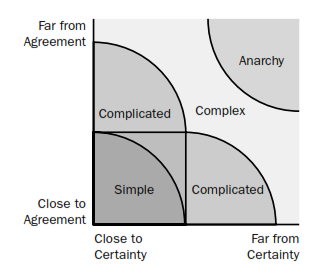
\includegraphics[width=0.6\textwidth]{./figures/complexity_assessment_graph.PNG}
  \caption{complexity assessment graph}
  \label{fig:ch1-complexity_assessment_graph}
\end{figure}\bigskip

The team takes a look at the requirements, considers the available technology, and evaluates its own skills and capabilities. It then collectively determines how to build the functionality.





\section{iterations}

\begin{itemize}
  \item At the start of an iteration, the team reviews what it must do. 
  \item It then selects what it believes it can turn into an increment of potentially shippable functionality by the end of the iteration
  \item team is then left alone to make its best effort for the rest of the iteration
  \item At the end of the iteration, the team presents so that the stakeholders can inspect and timely adaptations ca be made
\end{itemize}


\section{scrum roles}

Scrum implements this iterative, incremental skeleton through three roles.

All management responsibilities in a project are divided among these three roles.

\begin{enumerate}
  \item Product Owner
  \item Scrum Master
  \item Team
\end{enumerate}


\subsection{Product Owner}

\begin{itemize}
  \item achieves initial and ongoing funding for the project
  \item responsible for representing the interests of everyone with a stake in the project and its resulting system.
  \item responsible for using the Product Backlog (glossary) so that valuable functionality is produced first.
  \item responsible to those funding the project for delivering the vision in a manner that maximizes their ROI, he formulates a plan for doing so that includes a Product Backlog
\end{itemize}


\subsection{Scrum Master}
\begin{itemize}
  \item responsible for the Scrum process, for teaching Scrum to everyone involved in the project
  \item implementing Scrum so that it fits within an organization’s culture and still delivers desired benefits
  \item ensuring that everyone follows Scrum rules and practices
\end{itemize}

The people who fill these roles are those who have committed to the project.

After the Sprint review and prior to the next Sprint planning meeting, the ScrumMaster holds a Sprint retrospective meeting with the Team


\subsection{Team}

\begin{itemize}
  \item responsible for developing functionality
  \item self-managing, self-organizing, and cross-functional
  \item responsible for figuring out how to turn Product Backlog into an increment of functionality within an iteration
  \item collectively responsible for the success of each iteration and of the project as a whole
\end{itemize}

Team tells the Product Owner how much of what is desired it believes it can turn into functionality over the next Sprint.


\subsection{two groups}
important distinction in scrum
\begin{itemize}
  \item 'chickens': are intereseted in the project, but not on the hook
  \item 'pigs': are on the hook
\end{itemize}

It should always be clear who is on the hook and who is just a kibitzer.

Who is responsible for the ROI, and who has a stake in the ROI but isn’t accountable?

The rules of Scrum distinguish between the chickens and the pigs to increase productivity, create momentum, and put an end to floundering. 

\section{scrum flow}

\subsection*{sprints}

All work is done in Sprints, each Sprint is an iteration of 30 consecutive calendar days.

Each Sprint is initiated with a Sprint planning meeting, where the Product Owner and Team get together to collaborate about what will be done for the next Sprint.

Selecting from the highest priority Product Backlog, the Product Owner tells the Team what is desired.



\subsection*{sprint planning}

Sprint meeting should not last longer than 8 hours.

The Sprint planning meeting has two parts: 

\begin{itemize}
  \item first four hours
  \begin{itemize}
    \item are spent with the Product Owner presenting the highest priority Product Backlog to the Team
    \item The Team questions him or her about the content, purpose, meaning, and intentions of the Product Backlog
    \item When the Team knows enough, selects as much Product Backlog as it believes it can turn into a completed increment of potentially shippable product functionality by the end of the Sprint.
  \end{itemize}
  \item second four hours
  \begin{itemize}
    \item the Team plans out the Sprint
    \item The tasks that compose this plan are placed in a Sprint Backlog
    \item the tasks in the Sprint Backlog emerge as the Sprint evolves
  \end{itemize}
\end{itemize}

directly after the meeting, the sprint has started, 30 day target is tried to be met.



\subsection*{daily scrum}

Every day, the team gets together for a 15-minute meeting called a Daily Scrum.

each Team member answers three questions:

\begin{itemize}
  \item What have you done since last Daily Scrum?
  \item What do you plan on doing between now and next Daily Scrum?
  \item What impediments stand in the way of you meeting your commitments to this Sprint and this project? 
\end{itemize}

purpose of the meeting is to
\begin{itemize}
  \item synchronize each team member daily
  \item to schedule any meetings that the Team needs to forward its progress
  \item keeps all team activities visible so that the ScrumMaster can enforce the rules and help the team stay on track.
\end{itemize}



\subsection*{review meeting}

At the end of the Sprint a Sprint review meeting is held, it is an informal meeting.

four-hour meeting at which the Team presents what was developed during the Sprint to the Product Owner and any other stakeholders

purpose of the meeting is to
\begin{itemize}
  \item functionality is presented is intended to bring people together
  \item collaboratively determined what the Team should do next
\end{itemize}


\subsection*{Sprint retrospective}
After the Sprint review and prior to the next Sprint planning meeting, the ScrumMaster holds a Sprint retrospective meeting with the Team. three-hour meeting: revise the Teams development process to make it more effective and enjoyable for the next Sprint. 

\begin{figure}[H]
  \centering
  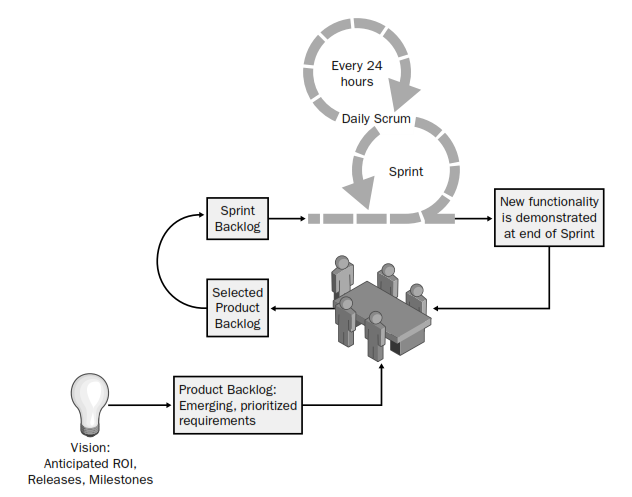
\includegraphics[width=0.6\textwidth]{./figures/chapter_1/scrum_process_overview.PNG}
  \caption{scrum process overview}
  \label{fig:ch1-scrum_process_overview}
\end{figure}\bigskip




\section{scrum artifacts}

\subsection{product backlog}
\begin{itemize}
  \item the Product Backlog is a list of functional and nonfunctional requirements
  \item it will deliver the vision of maximizing the ROI (glossary)
  \item is prioritized so that the items most likely to generate value are top priority and is divided into proposed releases
  \item changes in the Product Backlog reflect changing business requirements and how quickly or slowly the Team can transform Product Backlog into functionality.
  \item it is never complete
  \item is merely an initial estimate of the requirements
  \item is dynamic, evolves as the product and the environment does
  \item provides the Product Owner with a powerful tool for directing the project, giving the highest priority to the requirements that are of highest value to the business
  \item one of the purposes of the plan is to convince someone to fund the project, it should provide sufficient details to satisfy a source of funding that the project has merit, that it will deliver certain things at certain times, that the benefits outweigh the costs and risks, and that the people who will staff the project are sufficiently compentent to execute the plan
\end{itemize}

\begin{figure}[H]
  \centering
  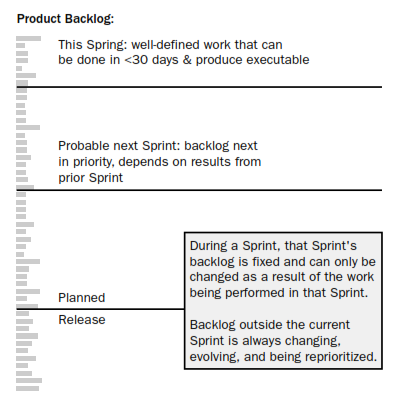
\includegraphics[width=0.6\textwidth]{./figures/product_backlog.PNG}
  \caption{product backlog}
  \label{fig:product_backlog}
\end{figure}\bigskip


\subsection{Sprint Backlog}
\begin{itemize}
  \item defines the work, or tasks, that a Team defines for turning the Product Backlog it selected for that Sprint into an increment of potentially shippable product functionality.
  \item Team compiles an initial list of these tasks in the second part of the Sprint planning meeting
  \item each takes should take roughly 4 to 16 hours to finish
  \item tasks taking longer than 4 to 16 hours are considered mere placeholders for tasks
  \item real-time picture of the work that the Team plans to accomplish
\end{itemize}


\subsection{Increment of Potentially Shippable Product Functionality}
\begin{itemize}
  \item Scrum requires Teams to build an increment of product functionality every Sprint
  \item this increment must be \textbf{potentially shippable}
  \item therefore increment should consist of thoroughly tested, well-structured, and well-written code
  \item user operation of the functionality is documented
\end{itemize}




 

\pagebreak
\chapter{New Management Responsibilities}

all three management roles are 'pig' roles: Product Owner, ScrumMaster, and Team. All other
managers in an organization are 'chickens', they all have to work through the pigs.
Chickens have no direct authority over the project’s execution or progress. Scrum management is responsible for inspecting the aspects of the project that Scrum makes visible and adapting accordingly.

Developers need to focus on producing the product. 

Sales and marketing want quick responses to every opportunity that comes knocking.

Scrum helps to balance the needs of both the marketing and the development departments.

Scrum banns interference during the Sprint, everyone else must leave the developers alone to work $\rightarrow$ redirected to higher priority work at the Sprint planning meeting.

Traditionally, customers get to state the requirements that optimize their ROI at the start of the project, but they don’t get to assess the accuracy of their predictions until the project is completed. Scrum lets the Product Owner adjust the ROI much more frequently.

In a huge reversal of ordinary management practices, Scrum makes the team responsible for managing development activities. Traditionally, the project manager tells the team what to do and manages its work.

The pressure inherent in a 30-day Sprint, the commitment the team members make to each other to accomplish something, and the principles of selforganization and cross-functional responsibilities all help the team successfully fulfill this responsibility.

When anyone outside the team tries to tell the team what to do, more damage than good usually results.

Teams that are too big dont work effectively, a team should optimally have 7 members.


Scrum is structured to regularly make the state of the project visible to the three managers—the Product Owner, the ScrumMaster, and the Team—so that they can rapidly adjust the project to best meet its goals.






 

\pagebreak
\chapter{the scrum master}
\label{sec:the_scrum_master}

The ScrumMaster is responsible for the success of the project, and he or she helps increase the probability of success by helping the Product Owner select the most valuable Product Backlog and by helping the Team turn that backlog into functionality. The ScrumMaster earns no awards or medals because the ScrumMaster is only a facilitator. 

Scrum involves a paradigm shift from control to empowerment, from contracts to collaboration, and from documentation to code.

People often hire consultants because they want to get a different perspective on their situations. This new perspective is often perceived as somehow better than the native view of things.


\subsection*{The shift from project manager to ScrumMaster}
\begin{itemize}
  \item shift from controlling to facilitating
  \item from bossing to coaching
  \item from manager to leader
  \item from authority to no authority
  \item from delegating to being personally responsible
  \item from controlling to guiding
\end{itemize}

The ScrumMaster’s job is to protect the team from impediments during the Sprint. However, the ScrumMaster has to operate within the culture of the organization. The ScrumMaster walks a fine line between the organization’s need to make changes as quickly as possible and its limited tolerance for change. 

Whenever possible, the ScrumMaster makes a  case and pushes the necessary changes through. The results are often greater productivity and greater return on investment (ROI). However, sometimes these changes are culturally unacceptable and the ScrumMaster must acquiesce.

Whenever an opportunity arises that was more important than the work selected by the team for the Sprint, management can abnormally terminate the Sprint. The Team, the Product Owner, and management would then conduct a new Sprint planning meeting. The new opportunity would be selected if it truly was the top-priority Product Backlog. Scrum keeps everything highly \textbf{visible}. By keeping everything in full view, the type of backroom politicking and influence swapping normal in most organizations is minimized.


The responsibilities of the ScrumMasters can be summarized as follows:
\begin{itemize}
  \item Remove the barriers between development and the Product Ownerso that the Product Owner directly drives development.
  \item Teach the Product Owner how to maximize ROI and meet his or herobjectives through Scrum.
  \item Improve the lives of the development team by facilitating creativityand empowerment.
  \item Improve the productivity of the development team in any way possible.
  \item Improve the engineering practices and tools so that each incrementof functionality is potentially shippable.
  \item Keep information about the team’s progress up-to-date and visible toall parties.
\end{itemize}

These responsibilities should be enough to keep the ScrumMaster busy; no ScrumMaster should have any time left over to act like a typical boss. ScrumMaster who acts like a program manager probably isn’t fulfilling all of his or her  duties as a ScrumMaster.




 

\pagebreak
\chapter{bringing order from chaos}

keywords: 
\begin{itemize}
  \item time-boxing
  \item incremental delivery
  \item practice of empowerment
  \item self-organization
\end{itemize}

Problems in many organizations: The people who analyzed the situation and set requirements were not the same people who would design the solutions that met these requirements. The people who designed these solutions were not the same people who would code the solutions. 

It can be hard trying to figure out every thing in advance in a complex project. The developers dont have enough time both to build functionality and to debug it. By focusing on \textbf{increments of functionality}, the team makes orderly  progress toward completing the release. Since each increment is tested as it is coded, the number of bugs never overwhelms the project. Scrum’s requirement that each increment of code be potentially shippable requires the  incremental removal of defects and minimizes ongoing bugs.

When using Scrum, teams are empowered to find their own way through \textit{complex situations}.

A Scrum of Scrums (glossary) is the usual mechanism that coordinates multiple teams working on a single project, much as the Daily Scrum is the mechanism that coordinates the work of multiple people on a single team. The work of many teams is coordinated by individuals from each of the teams.

Before a project officially begins, the planners of the project parse the work among teams to minimize dependencies.Teams then work on parts of the project architecture that are orthogonal to each other. This coordination mechanism is effective only when there are minor couplings or dependencies that require resolution, otherwise this wont work.

Sometimes projects are so complex that they require something more than the normal implementation of Scrum. As the degree of complexity rises, the number of inspections must be increased. Because of the increased frequency of inspections, the opportunity for adaptation also increases. The usual Daily Scrum wouldn’t offer enough opportunities for inspection of progress and detection of dependencies at play, and inspection is required for the necessary adaptations to be selected and implemented.

Out-of-the-box Scrum doesn’t have practices that address the complexities of every project. However, ScrumMasters have only to refer back to Scrum theory to find Scrum practices that can be readily adapted to handle even the most complex projects.

For complex projects
\begin{itemize}
  \item reduce the complexity to a degree where the team can cope and function
  \item focus on the next 30 calendar days
  \item forget the rest of the release and to focus on a few concrete steps, the rest falls into place
  \item staff the teams so that all the expertise necessary to develop a piece of functionality was included within each team. Each team will be able to resolve any dependencies it had on other teams. Most members of each team were able to focus on the work at hand, while the cross-team members spent time synchronizing team progress with that of other dependent teams.
\end{itemize}

This enables the team to focus and implement the foundation upon which the rest of the release and future Sprints depend. 

\pagebreak
\chapter{the product owner}


\begin{itemize}
  \item face-to-face communication over documentation
  \item collaboration over reports
\end{itemize}

Downplaying Scrum can simplify collaboration by reducing the overhead of learning something new and the apprehension of a strange new methodology. A Product Backlog could just be a prioritized list of requirements and a month the time between meetings.


A key element in scrum is that Team and the Product Owner need to learn to understand each other.
The Product Owner learns to talk in terms of business requirements and objectives, whereas the Team learns to speak in terms of technology. Because the Product Owner is unlikely to learn the technology, one of the main jobs of the ScrumMaster is to teach the Team to talk in terms of business needs and objectives.

The common denominator between the Team and the Product Owner is the Product Backlog. 

The ScrumMaster can get the Product Owner and the Team to speak the same language, to use a meaningful common vocabulary to discuss a mutual problem. He needs to understand the depths of the language divide that potentially separates customers and developers. Bridging this gap is critical; if both sides can't speak the same language, collaboration can't and won't occur.

The Product Owner has no interest in bridging the gap, and doesn't have the background to do so anyway, so it is up to the ScrumMaster to help the Team bridge the gap.

 

\pagebreak
\chapter{Planning a Scrum Project}

The Scrum planning process sets stakeholders’ expectations. These stakeholders include those who fund the project, those who intend to use the functionality created by the project, and those who will be otherwise affected by the project. The plan is a way of synchronizing stakeholders’ expectations with the Team’s expectations.

At the end of the Sprint, the stakeholders attend the Sprint review meetings and compare the project’s actual progress against its planned progress.

Changes in course and revisions to the plan made in Sprint planning meetings are explained to the stakeholders.

For those who are unable to attend the Sprint review meeting, the project reports compare actual results to the plan—both the original plan and the plan as it has been modified since the project’s inception.

The Scrum planning process involves resolving three questions:

\begin{itemize}
  \item What can those funding the project expect to have changed when the project is finished?
  \item What progress will have been made by the end of each Sprint?
  \item Why should those being asked to fund the project believe that the project is a valuable investment, and why should they believe that those proposing the project can deliver those predicted benefits?
\end{itemize}


Scrum projects require less planning than typical Gantt chart–based projects because those working to deliver the expected benefits provide visibility into their progress at the end of every Sprint.


The minimum plan necesary to start a Scrum project consists of a vision and a Product Backlog.

The vision describes why the project is being undertaken and what the desired end state is. For a system used internally within an organization, the vision might describe how the business operation will be different when the system is installed. For software that is being developed for external sale, the vision might describe the software’s major new features and functions, how they will benefit customers, and what the anticipated impact on the marketplace will be.

The Product Backlog defines the functional and nonfunctional requirements that the system should meet to deliver the vision, prioritized and estimated. It is parsed into potential sprints.





\subsection{implementing scrum in running projects}

Scrum is often implemented well after the project in question has been planned. In the case of these projects, the funding is already in place and expectations have already been established. What’s necessary  ow is to replan the project in light of Scrum so that the Team, Product Owner, and stakeholders can envision the project as a series of Sprints that lead to a release, all driven by the Product Backlog.


The first task is to create the Scrum artifact needed for managing a Scrum project: the Product Backlog.

\subsection{Estimating the Product Backlog}

To estimate each requirement precisely, one would have to know the exact composition and interaction of the requirement, the technology used to build the requirement, and the skills and mood of the people doing the work. One could potentially spend more time trying to define these attributes and their interactions than we would spend actually transforming the requirement into functionality.

The nature of complex problems is such that very small variations in any aspect of the problem can cause extremely large and unpredictable variations in how the problem manifests itself.

The purpose of estimating is to get a handle on the size of each requirement, both in its own right and relative to the size of the other requirements.

This information helps prioritize the Product Backlog and divide it into Sprints.

Scrum is empirical and ultimately based on the “art of the possible.” The team only has to do its best during each Sprint, and the expectations about what could be done are upated by the end of each Sprint.
Actual progress is being tracked on each sprint's product backlog. At the end of every Sprint, expectations are updated by tracking actual delivery of functionality against expected delivery of functionality.

estimates should include
\begin{itemize}
  \item how long it would take to analyze, design, and code the requirements
  \item time for unit testing, test automation
  \item time for code reviews, for refactoring, for writing code cleanly and legibly, and for removing unnecessary code
\end{itemize}


\subsection{What Does 'Done' Mean?}

 

\section*{quotations}


\begin{quotation}
  Scrum hangs all of its practices on an iterative,  process skeleton. The heart of Scrum lies in the iteration.
\end{quotation}


\begin{quotation}
  Scrum addresses the complexity of software development projects by implementing the inspection, adaptation, and visibility requirements of empirical process control with a set of simple practices and rules, which are described in the following sections. 
\end{quotation}


\begin{quotation}
  The people who fill these roles are those who have committed to the project ('pigs'). Others might be interested in the project, but they aren’t on  he hook. Scrum makes a clear distinction between these two groups and ensures that those who are responsible for the project have the authority to do what  s necessary for its success and that those who aren’t responsible can’t interfere unnecesarily ('chickens'). 
\end{quotation}


\begin{quotation}
  All work is done in Sprints
\end{quotation}


\begin{quotation}
  
\end{quotation}


\begin{quotation}
  
\end{quotation}


\begin{quotation}
  
\end{quotation}


\begin{quotation}
  
\end{quotation}


\begin{quotation}
  
\end{quotation}


\begin{quotation}
  
\end{quotation}


\begin{quotation}
  
\end{quotation}


\begin{quotation}
  
\end{quotation}


\begin{quotation}
  
\end{quotation}


\begin{quotation}
  
\end{quotation}


\begin{quotation}
  
\end{quotation}


\begin{quotation}
  
\end{quotation}

 

\section*{glossary}

\begin{table}[H]
  \begin{tabular}{lll}
    \textbf{burndown chart} &  shows the amount of work remaining across time, the correlation between amount of work remaining and the progress of the Team(s) in reducing it\\
    \textbf{'chicken'} &  someone in the project which role implies that he is not 'on the hook'\\
    \textbf{defined process control} &  Laying out a process that repeatably will produce acceptable quality output\\
    \textbf{Daily Scrum} & team gets together for a 15-minute meeting\\
    \textbf{empirical process control} &  When defined process control cannot be achieved because of the complexity of the intermediate activities\\
    \textbf{functional /non-functional requirements} &  While functional requirements define what the system does or must not do, non-functional requirements specify how the system should do it\\
    \textbf{management roles} & Product Owner, ScrumMaster, and Team (all three 'pigs')\\
    \textbf{product Backlog} & The list of functional and nonfunctionalrequirements\\
    \textbf{'pig'} & someone in the project which role implies that he is 'on the hook'\\
    \textbf{ROI} &  return on investment\\
    \textbf{Scrum of Scrums} &  the work of many teams is coordinated by individuals from each of the teams.\\
    \textbf{stakeholders} &  those with an interest in the software and how it works, who fund the project, those who intend to use the functionality created by the project, and those who will be otherwise affected by the project\\
   & 
  \end{tabular}
\end{table} 



\end{document} 